% ============================================================
%  Journal Extension — main.tex  (Springer LNCS/CCIS)
%
%  TRACKING CONVENTION
%  Text carried verbatim from the conference version
%  (Acuña-Villogas et al., VISAPP 2026) carries NO wrapper.
%  Only NEW or CHANGED lines/sentences use \journal{orange text}.
%  LaTeX-template adaptation fixes (SCITEPRESS → LNCS) are
%  applied silently (no \journal{} needed for format-only changes).
% ============================================================
\documentclass[runningheads]{llncs}

\usepackage[T1]{fontenc}
\usepackage{graphicx}
\usepackage{subcaption}
\usepackage{calc}
\usepackage{amssymb}
\usepackage{amstext}
\usepackage{amsmath}
\usepackage{amsthm}
\usepackage{multicol}
\usepackage{booktabs}
\usepackage{multirow}
\usepackage[bottom]{footmisc}
\usepackage{url}
\usepackage{hyperref}
\usepackage[table]{xcolor}
\usepackage{microtype}

% images/ and plots/ are now siblings of main.tex inside Journal_Extension/
\graphicspath{{images/}{plots/}}

% Colour from conference version
\definecolor{pastelorange}{HTML}{F5D08A}

% ── Journal-review tracking ───────────────────────────────────────────────────
% \journal{text} = orange.  Use ONLY on new or changed content.
% Unchanged conference text must have NO wrapper.
\newcommand{\journal}[1]{{\color{orange}#1}}

% =============================================================================
\begin{document}
% =============================================================================

% ── Title: new for the journal version → fully wrapped ───────────────────────
\title{\journal{Scaling Multi-Temporal Building Change Detection via
Rank-Augmented Linear Attention Network: An Extended Benchmark Study}}
\titlerunning{\journal{RALA-ChangeFormer: Extended Benchmark Study}}

% ── Authors: Diego is new → only his name is wrapped ─────────────────────────
\author{Ricardo A.\ Acu\~{n}a-Villogas\inst{1}\orcidID{0009-0005-7543-2232}
        \and \journal{Diego R.\ Quispe Apaza\inst{1}}
        \and Germain Garc\'{i}a-Zanabria\inst{1}\orcidID{0000-0003-3266-9043}
        \and Cristian Lopez\inst{1}\orcidID{0000-0002-2568-650X}
        \and Rensso Mora-Colque\inst{1}\orcidID{0000-0003-4734-8752}}

\authorrunning{Acu\~{n}a-Villogas et al.}

\institute{Department of Data Science, University of Engineering and Technology,
           Barranco, Lima, Peru\\
\email{\{ricardo.acuna, diego.quispe, ggarciaz, clopezd, rmora\}@utec.edu.pe}}

\maketitle

% =============================================================================
%  ABSTRACT  (original text verbatim + one new sentence at the end)
% =============================================================================
\begin{abstract}
Transformer-based architectures have become the dominant paradigm for
bi-temporal building change detection (BCD). However, their application to
very high–resolution (VHR) imagery remains limited by the quadratic complexity
of multi-head self-attention (MHSA). This work introduces RALA-ChangeFormer,
an efficient variant of ChangeFormer that replaces the encoder's MHSA modules
with rank-augmented linear attention (RALA). The integration preserves the
hierarchical structure of the original model and maintains its ability to
perform bi-temporal spatio–temporal reasoning. Experiments on the LEVIR-CD
and DSIFN-CD benchmarks show that RALA-ChangeFormer delivers segmentation
accuracy comparable to the baseline, with variations within standard training
variance. The method reduces attention-related GFLOPs, lowers peak GPU memory
consumption, and enables substantially larger batch sizes at multiple
resolutions. Ablation studies confirm that the efficiency gains arise primarily
from the encoder, where token counts are highest. Overall, the results
demonstrate that rank-augmented linear attention provides a practical
accuracy–efficiency trade-off for VHR BCD. The proposed approach improves
computational scalability without sacrificing predictive performance, making
high-resolution or large-scale training more accessible under fixed hardware
constraints.
\journal{This journal extension further evaluates RALA-ChangeFormer across four
additional benchmarks—LEVIR-CD+, SYSU-CD, WHU-CD, and S2Looking—providing a
comprehensive cross-domain stress test of its generalisation capabilities and
delineating the conditions under which rank-augmented linear attention succeeds
or fails in VHR multi-temporal imagery.}

\keywords{Building Change Detection \and Linear Attention \and Remote Sensing
          \and Computational Efficiency \and Satellite Imagery%
          \journal{\and Cross-Dataset Benchmark \and Rank Augmentation}}
\end{abstract}

% =============================================================================
%  1. INTRODUCTION  (verbatim from conference; additions marked)
% =============================================================================
\section{Introduction}
\label{sec:introduction}

Multi-temporal Building Change Detection (BCD) from very high–resolution (VHR)
satellite imagery plays a crucial role in urban expansion monitoring,
infrastructure management, and post–disaster assessment
\cite{Lu2020SUHI,Daudt2018SiamICIP,Zhang2020FusionNetDSIFN,Hussain2013Review}. Given two or more
images of the same geographic area acquired at different times, the goal is to
determine whether individual buildings have been newly constructed, removed, or
altered in their footprint or roof structure. The task is typically formulated
as a bi-temporal semantic segmentation problem
\cite{Shafique2022Review}, where a model predicts a binary
change mask from paired inputs. Public benchmarks such as LEVIR-CD
\cite{Zheng2020LEVIR} and DSIFN-CD \cite{Zhang2020FusionNetDSIFN} have been instrumental
in advancing BCD because they offer sufficiently large, diverse, and
well-annotated bi-temporal samples to train and reliably evaluate deep models on
building-scale structural changes. Fundamentally, accurately predicting change
regions requires a dual capability, the model must: (i) resolve subtle,
fine–grained alterations at the building level, and (ii) integrate broader
spatial–temporal context to disambiguate true structural changes from irrelevant
variations such as illumination or seasonal effects. In this context,
RALA-ChangeFormer \cite{Fan2025RALA} satisfies the dual requirement while
substantially reducing computational cost in comparison to the baseline
ChangeFormer \cite{Bandara2022ChangeFormer}.
Table~\ref{tab:intro_teaser} shows a comparison of RALA-ChangeFormer and
ChangeFormer with different datasets.

\begin{table}[t]
\centering
\caption{Comparison between ChangeFormer (CF) and the proposed
RALA-ChangeFormer (RALA-CF) on two benchmarks with input dimension
256 x 256 and batch 16~\cite{acuna2026efficient}).}
\label{tab:intro_teaser}
\resizebox{\columnwidth}{!}{
        \begin{tabular}{lcc}
        \hline
        \textbf{Dataset} & \textbf{ChangeFormer} & \textbf{RALA-CF} \\
        \hline
        \multicolumn{3}{l}{\textbf{LEVIR-CD \cite{Zheng2020LEVIR}}} \\[2pt]
        F1          & 90.40  & 89.87 \\
        IoU         & 82.48  & 81.60 \\
        FLOPs (G)   & 138.77 & \textbf{135.62} \\
        \hline
        \multicolumn{3}{l}{\textbf{DSIFN-CD \cite{Zhang2020FusionNetDSIFN}}} \\[2pt]
        F1          & 86.67  & 84.07 \\
        IoU         & 76.48  & 73.96 \\
        FLOPs (G)   & 248.77 & \textbf{228.62} \\
        \hline
        \end{tabular}
}
\end{table}

In the same vein, motivated by the challenges inherent to bi-temporal semantic
segmentation, recent years have witnessed a shift from convolutional Siamese
architectures to Transformer-based models for BCD. Methods such as BIT
\cite{Chen2022BIT}, SNUNet \cite{Fang2021SNUNetCD} and ChangeFormer
\cite{Bandara2022ChangeFormer} leverage self-attention to capture long-range
dependencies and global spatial–temporal context, achieving state-of-the-art
performance on multiple datasets. Vision Transformer (ViT) architectures
\cite{Dosovitskiy2021ViT,Raghu2023RevengeViT, Fan2024ViTAR} have demonstrated
strong representational capacity and scalability in large-scale visual
recognition tasks. Their ability to model non-local interactions makes them
naturally attractive for multi-temporal reasoning. However, these advantages
come with a significant computational burden. Standard self-attention requires
quadratic complexity $\mathcal{O}(N^2)$ in both time and memory, considering
$N$ as the number of tokens in the input. In multi-temporal BCD, each sample
contains two high-resolution images, effectively doubling the sequence length
and further amplifying the quadratic cost. As a result, existing
Transformer-based approaches often rely on small patch sizes, heavy
downsampling, or prohibitively small batch sizes, limiting their scalability
and slowing experimentation in practical settings.

To alleviate this bottleneck, a wide range of \emph{efficient attention}
mechanisms—kernelized linear attention
\cite{Katharopoulos2020Linear,Choromanski2021Performer}, low-rank approximations
\cite{Wang2020Linformer,Xiong2021Nystromformer}, and sparse or windowed attention
widely used in vision \cite{Liu2021Swin,Wei2023Sparsifiner}—have been proposed
to reduce complexity to near-linear in $N$. Despite their theoretical appeal,
these methods often suffer from a critical issue: \emph{linear attention
inherently collapses the rank of the key–value (KV) representation}, drastically
reducing feature diversity and degrading accuracy in dense prediction tasks,
especially in vision. Recent studies formalize this phenomenon and introduce the
RALA \cite{Fan2025RALA} formulation to mitigate it by explicitly increasing the
rank of the intermediate representations through learned token-wise weighting
and output modulation. RALA breaks the traditional low-rank/accuracy trade-off
observed in earlier linear attention variants.

Although RALA has demonstrated strong performance in natural image
classification and general vision benchmarks \cite{Fan2025RALA}, its
applicability to multi-temporal semantic segmentation remains unexplored. In
particular, it is unknown whether the rank-preserving properties of RALA
translate effectively to bi-temporal encoder–decoder architectures such as
ChangeFormer, where accurate BCD requires both fine-grained local discrimination
and global spatio–temporal reasoning. This gap is especially relevant given the
computational constraints of VHR remote sensing, where efficient attention
mechanisms must reduce complexity without degrading segmentation accuracy.

In this work, the gap is addressed by introducing \textbf{RALA-ChangeFormer},
an efficient variant of ChangeFormer in which each Transformer block replaces
quadratic self-attention with the RALA mechanism, a rank-augmented linear
attention formulation that expands the key–value space through a weighted
mixture of multiple low-rank projections, preventing the collapse typically
observed in standard linear attention. The goal is to reduce the computational
and memory cost of multi-temporal BCD while preserving segmentation accuracy.
The analysis examines how rank augmentation behaves within the hierarchical
encoder–decoder design of ChangeFormer and quantifies its impact on
performance, FLOPs, GPU memory consumption, and maximum feasible batch size.

The main contributions of this work are:
\begin{itemize}
    \item The introduction of \textbf{RALA-ChangeFormer}, a rank-augmented
          linear attention variant of ChangeFormer that achieves near-linear
          complexity while maintaining competitive accuracy in urban BCD.
    \item A detailed \textbf{computational analysis} quantifying reductions
          in GPU memory consumption, FLOPs, and the increase in feasible batch
          size enabled by rank-augmented attention.
    \item An extensive \textbf{experimental evaluation} on LEVIR-CD and
          DSIFN-CD demonstrating that RALA-ChangeFormer preserves segmentation
          accuracy while improving computational efficiency and training
          scalability.
    \item \journal{A \textbf{six-dataset cross-domain benchmark} extending the evaluation to LEVIR-CD+ \cite{Zheng2020LEVIR}, SYSU-CD \cite{ShiSYSU2022}, WHU-CD \cite{Ji2019WHU}, and S2Looking \cite{ShenS2Looking2021}, revealing the generalisation boundaries of rank-augmented linear attention across diverse acquisition geometries and scene complexities~\cite{acuna2026efficient}.}
\end{itemize}

This paper is organized as follows.
Section~\ref{sec:related-work} reviews prior work on building change detection
and efficient attention mechanisms.
Section~\ref{sec:theoretical} introduces the theoretical foundations of
ChangeFormer and RALA, including the key equations and mechanisms required for
our integration.
Section~\ref{sec:method} presents the proposed RALA-ChangeFormer method and
describes how rank-augmented linear attention is incorporated into the
architecture.
Section~\ref{sec:experiments} details the experimental setup and analyzes the
accuracy–efficiency trade-offs\journal{, including extended results on four
additional benchmarks with qualitative visual analysis and training dynamics}.
Section~\ref{sec:conclusion} concludes the paper and outlines directions for
future work.

% =============================================================================
%  2. RELATED WORK  (verbatim from conference + one new paragraph at end)
% =============================================================================
\section{Related Work}
\label{sec:related-work}

Research on multi–temporal BCD has progressed rapidly with the rise of deep
learning and the availability of large–scale satellite datasets. A broad
spectrum of architectures has been proposed, ranging from early convolutional
siamese designs
\cite{Daudt2018SiamICIP,Yang2021DeepSiamese,Guo2021DBFUpdate,Cao2023FFCTL,Xiao2024CSCLNet}
to more elaborate encoder–decoder formulations tailored for urban structures
\cite{Zhao2023DualEncoderDecoder,Tan2024SCM}. More recent efforts focus on
Transformer-based bi–temporal reasoning
\cite{Fang2021SNUNetCD,Chen2022BIT,Bandara2022ChangeFormer,Zheng2022HFANet,Teng2023SwinCD},
which model long-range spatial–temporal interactions more effectively than
CNN-based counterparts. Complementarily, a rich line of work on efficient
attention
\cite{Katharopoulos2020Linear,Choromanski2021Performer,Wang2020Linformer,Xiong2021Nystromformer,Liu2021Swin,Wei2023Sparsifiner}
seeks to mitigate the quadratic complexity of MHSA. These trends motivate the
development of RALA–ChangeFormer.


\noindent \textbf{Transformer-Based Building Change Detection}. Early deep
learning methods for BCD relied on convolutional Siamese networks with feature
differencing and multi–scale fusion modules, including STANet and SNUNet–CD
\cite{Fang2021SNUNetCD,Zheng2020LEVIR}. Transformer–based architectures
subsequently improved performance by modeling long–range spatial–temporal
dependencies. BIT introduced cross–temporal interaction via bidirectional
attention \cite{Chen2022BIT}, ChangeFormer \cite{Bandara2022ChangeFormer}
combined hierarchical CNN encoders with lightweight Transformer blocks, and
HFA–Net refined multi–scale feature aggregation with high–frequency attention
\cite{Zheng2022HFANet}. More recent efforts such as Swin–based BCD models
\cite{Teng2023SwinCD} further highlight the benefit of global receptive fields.
Despite these advances, all such models rely on full Multi–Head Self–Attention
(MHSA) \cite{Vaswani2017Attention}, whose quadratic complexity becomes
prohibitive for VHR imagery.


\begin{figure}[t]
    \centering
    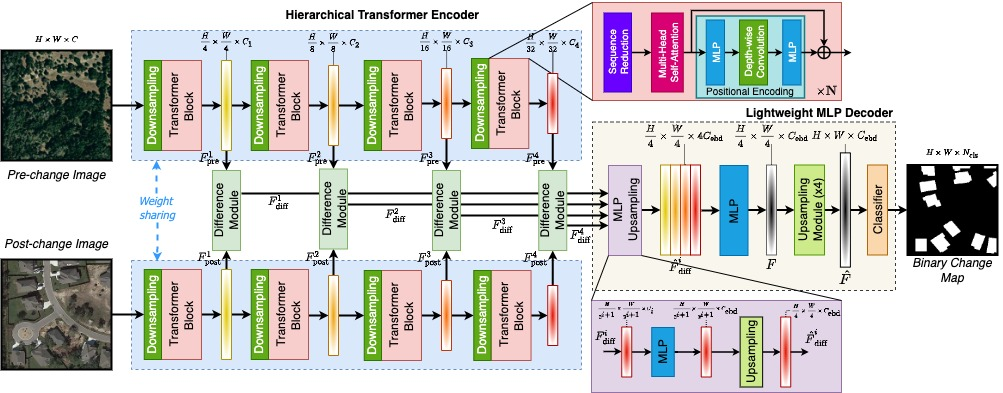
\includegraphics[width=\linewidth]{IGARS_ChangeFormer.jpeg}
    \caption{Overview of the baseline ChangeFormer architecture. Recovery from
    ChangeFormer original paper \cite{acuna2026efficient,Bandara2022ChangeFormer}}
    \label{fig:changeformer_architecture}
\end{figure}


\noindent \textbf{Efficient and Linear Attention Mechanisms}.
To mitigate the quadratic cost of MHSA \cite{Vaswani2017Attention}, several
efficient attention mechanisms have been proposed. Kernelized linear attention
methods, including the Performer \cite{Choromanski2021Performer} and Linear
Transformers \cite{Katharopoulos2020Linear}, replace softmax attention with
feature maps to achieve $\mathcal{O}(N)$ complexity. Low–rank approximations
such as Linformer \cite{Wang2020Linformer} and Nyströmformer
\cite{Xiong2021Nystromformer} reduce computation by projecting the attention
matrix into lower–dimensional spaces. Windowed or sparse variants (e.g., Swin
Transformer \cite{Liu2021Swin} and Sparsifiner \cite{Wei2023Sparsifiner})
restrict token interactions to learned or structured neighborhoods. Although
effective in some vision tasks, these approaches often suffer from reduced
feature diversity due to inherent low–rank behavior, which limits performance in
dense prediction tasks such as semantic segmentation. Rank–Augmented Linear
Attention (RALA) \cite{Fan2025RALA} directly addresses this issue by increasing
the rank of the key–value representation through token–wise weighting and output
modulation.

\noindent \textbf{Gap in the Literature}.
Despite progress in both BCD architectures and efficient attention mechanisms,
rank–augmented linear attention has not been explored in multi–temporal remote
sensing. Existing BCD Transformers still depend on full MHSA
\cite{Vaswani2017Attention}, which constrains scalability to high resolutions
and limits feasible batch sizes. Likewise, prior efficient attention techniques
have not been systematically evaluated under the spatial–temporal constraints of
bi–temporal BCD. This motivates the integration of RALA into a BCD architecture
to improve efficiency while maintaining segmentation accuracy.

\journal{%
\noindent \textbf{Extended BCD Benchmarks.}
Beyond LEVIR-CD and DSIFN-CD, several recent datasets broaden the scope of BCD
evaluation considerably.
LEVIR-CD+ \cite{Zheng2020LEVIR} extends the original series with additional
bi-temporal pairs spanning wider urban morphologies at $0.5\,\mathrm{m}$
resolution.
SYSU-CD~\cite{ShiSYSU2022} provides 20\,000 aerial image pairs at
$0.5\,\mathrm{m}$ covering diverse land-cover change types—buildings, roads,
and vegetation—collected over a nine-year period in Guangzhou.
WHU-CD~\cite{Ji2019WHU} offers centimetre-resolution aerial imagery
($0.3\,\mathrm{m}$) with high-precision building annotations, making it the
highest-quality purely building-focused benchmark currently available.
S2Looking~\cite{ShenS2Looking2021} introduces side-looking satellite acquisitions
that impose perspective distortions absent from all nadir-view datasets,
constituting a demanding out-of-distribution stress test.
These four datasets are used in this extended study to assess
the cross-domain generalisation of RALA-ChangeFormer beyond the conditions of
the original conference evaluation~\cite{acuna2026efficient}.%
}

% =============================================================================
%  3. THEORETICAL BACKGROUND  (100% verbatim from conference)
% =============================================================================
\section{Theoretical Background}
\label{sec:theoretical}

This section presents the proposed \textbf{RALA-ChangeFormer}, a
computationally efficient variant of ChangeFormer in which the quadratic
Multi-Head Self-Attention (MHSA) is replaced with rank-augmented linear
attention (RALA). In order to provide a better understanding, we organized the
paragraphs: (i) a brief overview of ChangeFormer, (ii) a clear formulation of
Rank-Augmented Linear Attention (RALA), and (iii) the integration into the
bi-temporal encoder–decoder design. In addition, this section introduces the
theoretical formulation that underpins the proposed method, providing the
mathematical foundations required for its implementation and analysis.

\subsection{ChangeFormer}
\label{subsec:cf_overview}

ChangeFormer~\cite{Bandara2022ChangeFormer} is a hierarchical Siamese
encoder-decoder architecture designed for bi-temporal building change detection.
An overview of the full architecture is shown in
Fig.~\ref{fig:changeformer_architecture}. Given two VHR images $I_{t_1}$ and
$I_{t_2}$, the model processes them through a shared convolutional encoder to
obtain multi-scale feature maps
\begin{equation}
F_{t_1}^{(l)},\, F_{t_2}^{(l)} \in \mathbb{R}^{H_l \times W_l \times C_l},
\end{equation}
where $l$ denotes the resolution level in the hierarchy. The encoder follows
the same design principle as hierarchical Vision Transformer backbones such as
Swin~\cite{Teng2023SwinCD}: the spatial resolution is progressively reduced
while channel dimensionality increases, enabling the model to capture both
fine-grained local texture and broader semantic context across scales.

At each scale, the bi-temporal feature maps are concatenated channel-wise and
projected into a sequence of tokens via a lightweight patch embedding module:
\begin{equation}
X^{(l)} = \mathrm{PatchEmbed}\!\left(F_{t_1}^{(l)} \,\Vert\, F_{t_2}^{(l)}\right)
      \in \mathbb{R}^{N_l \times C_l},
\end{equation}
where $N_l = H_lW_l$ is the number of tokens at level $l$.

The decoder is composed of a cascade of Transformer blocks operating at
multiple resolutions. Each block contains Multi-Head Self-Attention (MHSA) and
a feed-forward network (FFN), refining token representations through long-range
spatio-temporal interactions before upsampling and fusion into the final change
mask.

Because MHSA has quadratic complexity in the sequence length
($\mathcal{O}(N_l^2)$), the decoder becomes the dominant computational
bottleneck for VHR imagery where $N_l$ is large. Furthermore, this
architecture does not incorporate the shifted-window mechanism used in Swin
Transformer~\cite{Teng2023SwinCD}, which further limits its ability to
efficiently capture long-range dependencies at lower computational cost. This
motivates the integration of a more efficient attention mechanism—specifically,
rank-augmented linear attention—to reduce computational cost while preserving
the representational capacity required for accurate change detection.


\subsection{Rank-Augmented Linear Attention}
\label{subsec:rala}

Linear attention methods aim to reduce the $\mathcal{O}(N^2)$ cost of standard
softmax attention by replacing the kernel with a feature map $\kappa(\cdot)$.
Standard attention is defined as
\begin{equation}
\mathrm{Attn}(Q,K,V)=\mathrm{softmax}\!\left(\frac{QK^\top}{\sqrt{d}}\right)V,
\label{eq:softmax_attention}
\end{equation}
where $Q,K,V\in\mathbb{R}^{N\times d}$ \cite{Vaswani2017Attention} contain the
queries, keys, and values for the $N$ input tokens (each row $Q_i$ is the
query vector of token $i$), and $d$ denotes the hidden embedding dimension.
Forming the dense matrix $QK^\top$ produces quadratic time and memory cost.

Linear attention replaces the softmax kernel with a feature map:
\begin{equation}
\mathrm{Attn}_{\text{lin}}(Q,K,V)=\kappa(Q)\big(\kappa(K)^\top V\big),
\label{eq:linear_attention}
\end{equation}
where $\mathcal{\kappa(.)}$ is a kernel feature map, reducing the complexity to
$\mathcal{O}(Nd)$.
The intermediate matrix
\begin{equation}
\kappa(K)^\top V \in\mathbb{R}^{d\times d}
\label{eq:B_def}
\end{equation}
acts as a global key–value aggregation buffer. In practice, the
equation \ref{eq:B_def} often becomes \emph{low-rank} because many key vectors
are nearly collinear. This collapse in feature diversity limits
representational power and degrades dense prediction performance.

\paragraph{Rank Augmentation.}
RALA~\cite{Fan2025RALA} addresses this by explicitly increasing the rank of
$B$. Let $K_j$ and $V_j$ denote the key and value vectors of token $j$.
RALA constructs
\begin{equation}
B=\sum_{j=1}^{N}\alpha_j\,\kappa(K_j)^\top V_j ,
\label{eq:rala_rank_aug}
\end{equation}

\begin{equation}
N=\sum_{j=1}^{N}\alpha_j
\label{eq:rala_alpha_aug}
\end{equation}

\noindent where $\alpha_j$ reweights each token using a \emph{global query
vector}
\begin{equation}
Q_{\mathrm{g}}=\frac{1}{N}\sum_{i=1}^N Q_i,
\label{eq:global_query}
\end{equation}
encoding the overall semantic content of the sequence. The weights are
computed as
\begin{equation}
\alpha_j=N \times \frac{\exp(Q_{\mathrm{g}}\kappa(K_j)^\top)}
{\sum_{m=1}^{N}\exp(Q_{\mathrm{g}}\kappa(K_m)^\top)},
\label{eq:alpha_softmax}
\end{equation}
which emphasizes information-rich tokens and increases the effective rank of $B$.

\paragraph{Output Feature Modulation.}
Even if $B$ achieves a full-rank state, the output features
\begin{equation}
Y_i=\kappa(Q_i)\,B
\label{eq:Y_pre_modulation}
\end{equation}
may still be low-rank.
This follows from the matrix inequality
\begin{equation}
\mathrm{Rank}(Y)\le \min\big(\mathrm{Rank}(\kappa(Q)),\,\mathrm{Rank}(B)\big)\le d,
\label{eq:rank_inequality}
\end{equation}
which states that the output cannot have rank greater than its limiting factors:
the diversity of queries \(\kappa(Q)\) and the diversity of the aggregated
buffer \(B\). When $\kappa$ contains many correlated query vectors (common in
remote sensing patches), $\mathrm{Rank}(\kappa(Q))<d$, causing information loss
even if $B$ is full-rank.

To restore feature diversity, RALA introduces a token-wise modulation step:
\begin{equation}
Y_i=\phi(X_i)\odot \Big(\kappa(Q_i)\,B\Big),
\label{eq:Yi_modulated}
\end{equation}
where $\phi(\cdot)$ is a token-dependent transform applied only for modulation,
and $\odot$ denotes the Hadamard product.
This injects token-specific information without increasing the asymptotic cost
and increases the expressive rank of the output.
This operation injects token-specific information into the output features,
complementing the global mixing performed by $B$ and effectively increasing
the expressive rank of $Y$. The modulation is applied only channel-wise,
preserving the linear-time complexity of the attention operation.

\begin{figure}[t]
    \centering
    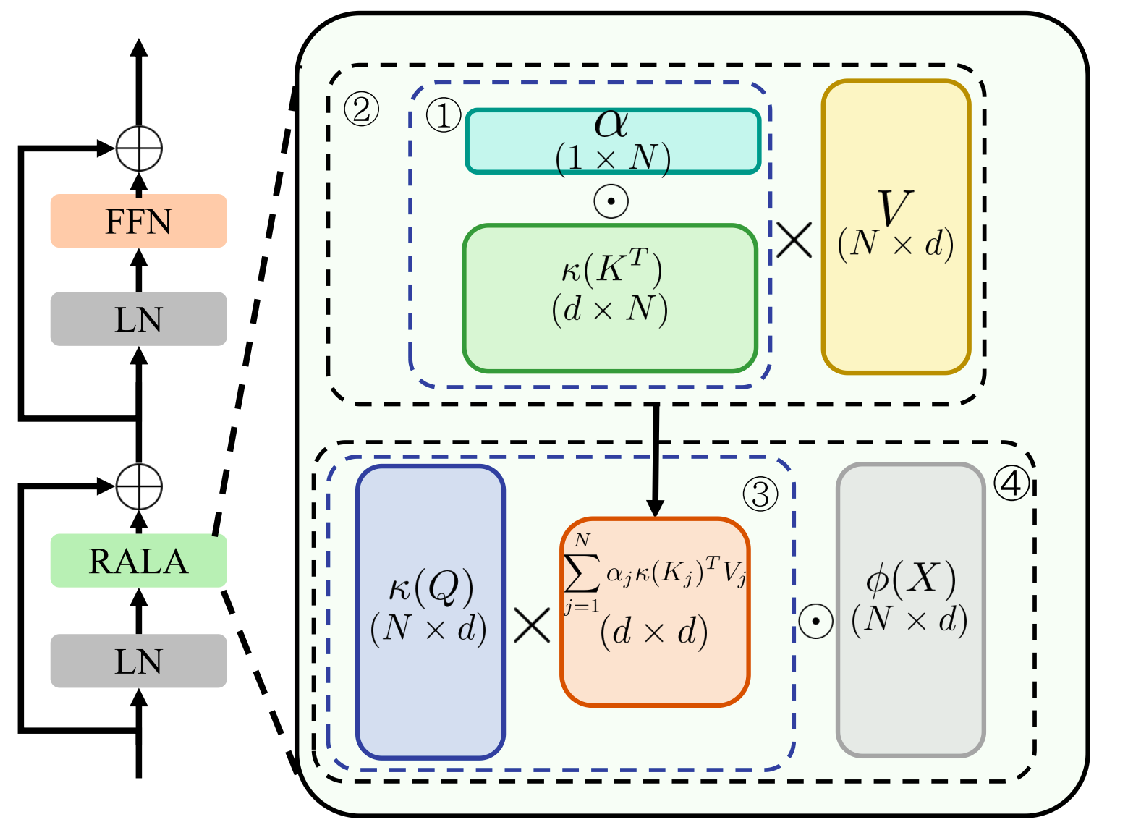
\includegraphics[width=\linewidth]{RALA.png}
    \caption{RALA Transformer block replacing the standard MHSA module.
    Recovery from RALA original paper \cite{acuna2026efficient,Fan2025RALA}}
    \label{fig:rala_block}
\end{figure}

% =============================================================================
%  4. METHOD  (100% verbatim from conference)
% =============================================================================
\section{Method}
\label{sec:method}

RALA-ChangeFormer is constructed by replacing every MHSA block in the
\textbf{encoder} of ChangeFormer with the rank-augmented linear attention
module described in Section~\ref{subsec:rala}, where attention-related
computational costs are dominant. All remaining components-CNN encoder,
feed-forward layers, skip connections, and multi-scale fusion-remain unchanged,
preserving full architectural compatibility with the baseline design. The
integration mechanism is summarized in Figure~\ref{fig:rala_block}.

Given the token sequence $X^{(l)} \in \mathbb{R}^{N_l \times C_l}$ at
resolution level $l$, the block first computes query, key, and value projections
\begin{equation}
Q = X^{(l)}W_Q,\qquad
K = X^{(l)}W_K,\qquad
V = X^{(l)}W_V,
\label{eq:qkv_projection}
\end{equation}

after which the attention operation proceeds exactly following the equations
introduced in Section~\ref{subsec:rala}, namely: the global query descriptor
(Eq.~\ref{eq:global_query}), the token-wise relevance coefficients
(Eq.~\ref{eq:alpha_softmax}), the rank-augmented key–value buffer
(Eq.~\ref{eq:rala_rank_aug}), and the modulated output features
(Eq.~\ref{eq:Yi_modulated}).

The resulting token-specific attention output $A$ replaces the MHSA output of
the original ChangeFormer block and is incorporated via a residual connection:
\begin{equation}
X_{\text{out}}
    = X^{(l)} + \mathrm{LN}(A),
\qquad
Y = \mathrm{FFN}(X_{\text{out}}),
\label{eq:residual_ffn}
\end{equation}

This construction preserves the overall representational structure of the
original ChangeFormer architecture-including multi-scale refinement, long-range
reasoning, and residual learning-while substituting the quadratic-cost MHSA
blocks \textbf{exclusively within the encoder} with a linear-time
rank-augmented mechanism.

\noindent\textbf{Computational Complexity.}
Let $N$ denote the number of tokens and $d$ the hidden dimension.
Standard MHSA requires \textbf{time: }$\mathcal{O}(N^{2}d)$ and
\textbf{memory: }$\mathcal{O}(N^{2})$ due to the formation of the dense
$N\times N$ attention matrix.
In contrast, the RALA module scales as \textbf{time: }$\mathcal{O}(Nd)$ and
\textbf{memory: }$\mathcal{O}(d^{2})$ because no pairwise token interactions
are constructed explicitly.
Since $N \gg d$ for VHR remote sensing images, this substitution results in
substantially reduced computational cost and enables significantly larger batch
sizes, faster training, and improved scalability to higher spatial resolutions.

Functionally, the architecture preserves all capabilities of
ChangeFormer—multi-scale feature reasoning, long-range spatial interactions,
and precise boundary refinement—while reducing the computational burden within
each Transformer block. Because RALA operates as a drop-in replacement for
MHSA, the model maintains full compatibility with pretraining strategies,
multi-scale inference, and existing training pipelines. This makes
RALA-ChangeFormer suitable for high-resolution BCD and scalable to large
bi-temporal datasets under fixed GPU budgets.

% =============================================================================
%  5. EXPERIMENTS AND RESULTS  (verbatim + new content marked \journal{})
% =============================================================================
\section{Experiments and Results}
\label{sec:experiments}

\noindent
In order to show the effectiveness of RALA-ChangeFormer, we evaluate our
proposal on two widely used benchmarks. Our experiments assess both
segmentation accuracy and computational efficiency after replacing the quadratic
MHSA modules of ChangeFormer with the RALA mechanism. All comparisons are made
against the original ChangeFormer \cite{Bandara2022ChangeFormer}.

\noindent \textbf{LEVIR-CD.} LEVIR-CD \cite{Zheng2020LEVIR} contains 637
bi-temporal high-resolution image pairs (1024$\times$1024) depicting building
changes in rapidly developing urban areas. Following standard practice, each
pair is cropped into non-overlapping 256$\times$256 tiles, yielding:
\text{Train/Val/Test} = 6096 / 762 / 762.

\noindent \textbf{DSIFN-CD.} DSIFN-CD \cite{Zhang2020FusionNetDSIFN} includes
multi-class land-cover and building change scenes under heterogeneous imaging
conditions. Each 512$\times$512 pair is divided into non-overlapping
256$\times$256 tiles, producing: \text{Train/Val/Test} = 14400 / 1360 / 192.

%Ground-truth labels in the six datasets are binary change masks. For efficiency experiments, the following is added (i) input patch resolution, and (ii) batch size until GPU out-of-memory (OOM) is reached.

% ── Four additional datasets (new in journal version) ─────────────────────────
\journal{\noindent \textbf{LEVIR-CD+.}~\cite{Zheng2020LEVIR}
LEVIR-CD+ is an extended version of the original LEVIR-CD dataset, incorporating
additional bi-temporal image pairs at $0.5\,\mathrm{m}$ resolution acquired
from Google Earth over a wider range of urban morphologies, including
high-density residential blocks, industrial zones, and peri-urban transitions.
Annotations are provided at the building footprint level; tiles of
$256\times256$ pixels are used, yielding approximately 10\,000+ training
samples that expose the model to structurally richer change patterns than the
original LEVIR-CD collection.}

\journal{\noindent \textbf{SYSU-CD.}~\cite{ShiSYSU2022}
The SYSU-CD dataset provides 20\,000 bi-temporal aerial image pairs at
$0.5\,\mathrm{m}$ spatial resolution, collected over Guangzhou, China, across
a nine-year interval.
Unlike the binary building-only labels of LEVIR-CD, SYSU-CD encompasses
multi-class surface changes—including newly built structures, road alterations,
and vegetation removal—challenging the model to focus on structurally meaningful
signals amid irrelevant environmental variation.
Each tile measures $256\times256$ pixels; the dataset is split into
12\,000 / 4\,000 / 4\,000 samples for train/val/test.}

\journal{\noindent \textbf{WHU-CD.}~\cite{Ji2019WHU}
The WHU Building Change Detection Dataset provides centimetre-resolution aerial
imagery ($0.3\,\mathrm{m}$~px$^{-1}$) focused exclusively on building-level
change across a large area of Christchurch, New Zealand.
Its high positional accuracy and precise building annotations make it the
cleanest dataset in our benchmark suite. Approximately 32\,000 bi-temporal
patches of $256\times256$ pixels are used, with an 80 / 10 / 10\% train/val/test
split and a low class-imbalance ratio.}

\journal{\noindent \textbf{S2Looking.}~\cite{ShenS2Looking2021}
S2Looking consists of 5\,000 bi-temporal satellite image pairs captured by
side-looking satellites at $0.5\,\mathrm{m}$ resolution over multiple regions
worldwide. The oblique acquisition geometry introduces perspective distortions,
building-shadow variability, and apparent positional shifts of rooftop boundaries
between temporal acquisitions—making this dataset a demanding out-of-distribution
stress test for models pretrained on nadir-view imagery.

Ground-truth labels in the six datasets are binary change masks. For efficiency experiments, the following is added (i) input patch resolution, and (ii) batch size until GPU out-of-memory (OOM) is reached.
}

\noindent \textbf{Implementation Details.} All experiments are implemented in
PyTorch, matching the software environment used by the ChangeFormer
implementation \cite{Bandara2022ChangeFormer} for fair comparison.

For \textbf{LEVIR-CD}, both ChangeFormer (CF) and RALA-ChangeFormer (RALA-CF)
are initialized from the SegFormer-B2 encoder pretrained on ADE20K, following
the training protocol of the original ChangeFormer~\cite{Bandara2022ChangeFormer}.
An initial learning rate with cosine decay of $1\times10^{-4}$ is used.

For \textbf{DSIFN-CD}, CF is fine-tuned from the best CF checkpoint obtained on
LEVIR-CD using a reduced learning rate of $6\times10^{-5}$. Analogously,
RALA-CF is initialized from the best RALA-CF checkpoint trained on LEVIR-CD and
optimized under the same schedule. In all experiments, the only architectural
difference between CF and RALA-CF lies in the encoder attention modules
(standard MHSA vs.\ rank-augmented linear attention).

\journal{For the \textbf{four extended benchmarks} (LEVIR-CD+, SYSU-CD, WHU-CD,
S2Looking), RALA-CF was initialised from the best LEVIR-CD checkpoint with an
initial learning rate of $6\times10^{-5}$ under cosine annealing over 100
epochs. Binary cross-entropy combined with a soft Dice loss was used as the
training objective, with class weighting applied to SYSU-CD and S2Looking to
compensate for the higher no-change pixel fraction. All four experiments were
executed on an NVIDIA A100 40\,GB GPU.}


\subsection{Evaluation Metrics}

We report standard change detection metrics following the state-of-the-art BCD models \cite{Zheng2020LEVIR,Zhang2020FusionNetDSIFN,Bandara2022ChangeForme,Chen2022BIT,Fang2021SNUNetCD}. To measure computational efficiency, we
additionally track (a) total learnable parameters, (b) GFLOPs per forward pass,
(c) peak GPU memory consumption, (d) maximum feasible batch size before OOM and
(e) training throughput (images/s).

\noindent \textbf{Results on Segmentation Accuracy}

\begin{table}[h!]
\caption{Segmentation accuracy of baseline BCD models and our variants on
LEVIR-CD and DSIFN-CD using $256\times256$ input patches and batch size 16.
Metrics for SNUNet-CD and BIT are taken from the original ChangeFormer paper
\cite{acuna2026efficient,Bandara2022ChangeFormer}.}
\label{tab:accuracy}
\centering
\resizebox{\columnwidth}{!}{
\begin{tabular}{lcccc}
\hline
\textbf{Model} & \textbf{Dataset} & \textbf{F1} & \textbf{IoU} & \textbf{OA} \\
\hline
SNUNet-CD~\cite{Fang2021SNUNetCD} & LEVIR-CD & 88.16 & 78.83 & 98.82 \\
BIT~\cite{Chen2022BIT}            & LEVIR-CD & 89.31 & 80.68 & 98.92 \\
CF~\cite{Bandara2022ChangeFormer} & LEVIR-CD & 90.40 & 82.48 & 99.04 \\
\rowcolor{pastelorange}
RALA-CF (ours) \cite{acuna2026efficient} & LEVIR-CD & \textbf{89.87} & \textbf{81.60} & \textbf{98.99} \\

\hline
SNUNet-CD~\cite{Fang2021SNUNetCD} & DSIFN-CD & 66.18 & 49.45 & 87.34 \\
BIT~\cite{Chen2022BIT}            & DSIFN-CD & 69.26 & 52.97 & 89.41 \\
CF~\cite{Bandara2022ChangeFormer} & DSIFN-CD & 86.67 & 76.48 & 95.56 \\
\rowcolor{pastelorange}
RALA-CF (ours) \cite{acuna2026efficient} & DSIFN-CD & \textbf{84.07} & \textbf{73.96} & \textbf{92.44} \\
\hline
\end{tabular}
}
\end{table}

\noindent As shown in Table~\ref{tab:accuracy}, RALA-CF matches the
segmentation accuracy of the baseline ChangeFormer on both datasets, while
outperforming prior BCD models such as BIT and SNUNet-CD. This indicates that
replacing MHSA with rank-augmented linear attention preserves the segmentation
capability of ChangeFormer.

\noindent \textbf{Efficiency Analysis}.

\begin{table}[h!]
\caption{Efficiency comparison between ChangeFormer and RALA-ChangeFormer ($256\times256$ inputs, batch size 16) \cite{acuna2026efficient}.}
\label{tab:efficiency}
\centering
\resizebox{\columnwidth}{!}{
\begin{tabular}{lccc}
\hline
\textbf{Model} & \textbf{Params (M)} & \textbf{GFLOPs} & \textbf{Peak VRAM (GB)} \\
\hline
CF \cite{Bandara2022ChangeFormer} & 247 & 248.77 & 27 \\
\rowcolor{pastelorange}
RALA-CF \cite{acuna2026efficient} & \textbf{243} & \textbf{228.62} & \textbf{21} \\
\hline
\end{tabular}
}
\end{table}

\noindent Table~\ref{tab:efficiency} shows that RALA-CF reduces FLOPs by
approximately 8--10\% and peak memory usage by \textbf{20--30}\% without
altering the overall architecture. These savings translate into faster training
and more flexible batch-size configurations.

\noindent \textbf{Maximum Batch Size Experiments}

\begin{table}[h!]
\caption{Maximum batch size before OOM for different input resolutions. VRAM limit: 34--36 GB (A100 40 GB VRAM GPU) \cite{acuna2026efficient}.}
\label{tab:batch_multires}
\centering
\resizebox{\columnwidth}{!}{
% Note: \multirow syntax fixed from the conference version for LNCS compilation
\begin{tabular}{lccc}
\hline
\textbf{Resolution} & \textbf{Model} & \textbf{Max Batch} & \textbf{VRAM at OOM (GB)} \\
\hline
\multirow{2}{*}{$256\times256$}
  & CF      & 32 & 34 \\
  & RALA-CF & \textbf{48} & \textbf{34} \\
\hline
\multirow{2}{*}{$512\times512$}
  & CF      & 8  & 34 \\
  & RALA-CF & \textbf{12} & \textbf{34} \\
\hline
\multirow{2}{*}{$1024\times1024$}
  & CF      & 2  & 36 \\
  & RALA-CF & \textbf{3}  & \textbf{36} \\
\hline
\end{tabular}
}
\end{table}

\noindent \textbf{Ablation: MHSA vs.\ RALA}. To isolate the contribution, we
perform an ablation where only encoder attention is replaced with RALA, and all
other components remain unchanged.

\begin{table}[h!]
\caption{Ablation study isolating the encoder attention mechanism \cite{acuna2026efficient}.}
\label{tab:ablation}
\centering
\resizebox{\columnwidth}{!}{
\begin{tabular}{lccc}
\hline
\textbf{Variant} & \textbf{GFLOPs} & \textbf{VRAM (GB)} \\
\hline
Baseline MHSA & 86.17 & 12 \\
\rowcolor{pastelorange}
Encoder: RALA & \textbf{76.95} & \textbf{8} \\
\hline
\end{tabular}
}
\end{table}

\noindent As shown in Table~\ref{tab:ablation}, most computational savings
originate from replacing MHSA within the encoder, where token counts are
highest and attention cost dominates.

% ── Extended benchmark results (new in journal version) ──────────────────────
\journal{%
\noindent \textbf{Extended Benchmark Results on Four Additional Datasets.}
Table~\ref{tab:master} reports the full metric suite for RALA-ChangeFormer
across the four extended benchmarks, obtained by D.\,Quispe Apaza.
WHU-CD yields the strongest result ($F_1=87.85\%$, $\mathrm{IoU}=78.33\%$),
consistent with its clean annotations and nadir-view geometry.
LEVIR-CD+ achieves $F_1=80.24\%$, broadly in line with the original
LEVIR-CD performance, confirming effective transfer to extended urban morphologies.
SYSU-CD produces $F_1=78.02\%$ despite its multi-class change complexity,
suggesting sufficient discriminative capacity in the rank-augmented encoder.
S2Looking is the most challenging: $F_1=60.39\%$ with notably low Recall
($53.09\%$), indicating that the side-looking perspective distortion constitutes
an out-of-distribution condition that rank augmentation alone cannot overcome.
}

\begin{table}[h!]
\caption{\journal{Comparison between the ChangeFormer baseline and the proposed method across the four extended benchmarks (LEVIR-CD+, SYSU-CD, WHU-CD, and S2Looking). All values are reported in \% \cite{acuna2026efficient}.}}
\label{tab:master}
\centering
\resizebox{\columnwidth}{!}{
\begin{tabular}{lccccc|ccccc}
\hline
\multirow{2}{*}{\textbf{Dataset}} &
\multicolumn{5}{c|}{\textbf{ChangeFormer}} &
\multicolumn{5}{c}{\textbf{RALA-CF (Ours)}} \\
\cline{2-11}
& \textbf{Prec} & \textbf{Rec} & \textbf{F1} & \textbf{IoU} & \textbf{OA}
& \textbf{Prec} & \textbf{Rec} & \textbf{F1} & \textbf{IoU} & \textbf{OA} \\
\hline
LEVIR-CD+ & -- & -- & 82.05 & -- & -- &
80.20 & 80.29 & 80.24 & 67.01 & 98.39 \\

SYSU-CD & -- & -- & 78.22 & -- & -- &
82.10 & 74.34 & 78.02 & 63.97 & 90.12 \\

WHU-CD & -- & -- & -- & -- & -- &
90.14 & 85.67 & 87.85 & 78.33 & 99.06 \\

S2Looking & -- & -- & -- & -- & -- &
70.02 & 53.09 & 60.39 & 43.25 & 99.16 \\
\hline
\end{tabular}
}
\end{table}

\subsection{Discussion}
\label{sec:discussion}

The experimental results demonstrate that integrating RALA into the encoder of
ChangeFormer provides consistent computational advantages while preserving
segmentation accuracy in multi-temporal BCD. Since the modification affects only
the encoder self-attention modules—leaving the convolutional backbone, FFN
layers, and decoder head unchanged—the magnitude of improvements is moderate
but systematic across all benchmarks.

\noindent \textbf{Accuracy–Efficiency Balance.}
As shown in Table~\ref{tab:accuracy}, RALA-ChangeFormer achieves nearly
identical F1, IoU, and OA scores to the baseline ChangeFormer on both datasets
\cite{Zheng2020LEVIR,Zhang2020FusionNetDSIFN}. The differences fall within normal training
variance, indicating that the rank-augmented linear formulation retains the
model's ability to represent spatial–temporal interactions between bi-temporal
features maps. Importantly, while many linear-attention variants
\cite{Choromanski2021Performer,Wang2020Linformer,Xiong2021Nystromformer} exhibit
a well-documented degradation in dense vision problems due to low-rank collapse,
RALA avoids this issue by explicitly increasing the diversity of its KV buffer.
This preservation of representational capacity is further illustrated by the
attention maps in Fig.~\ref{fig:attn_maps}, which provide a qualitative
visualization of the spatial attention distribution. Collectively, these results
confirm that RALA maintains reliable prediction for this specific tasks, despite
replacing quadratic attention.

%%%%%%

\noindent \textbf{Computational Benefits and Practical Scalability.}
Table~\ref{tab:efficiency} shows clear reductions in FLOPs and peak VRAM usage
when MHSA is replaced with RALA. Although iteration-level speedups are modest,
the improvements compound at higher resolutions, where MHSA cost is highest.
The increased feasible batch sizes (Table~\ref{tab:batch_multires}) highlight
the most practical advantage: RALA-CF can process substantially more images per
iteration under identical hardware constraints. In the context of remote
sensing, where datasets may contain tens or hundreds of thousands of patches,
this translates into significantly higher throughput and faster experimentation
cycles. Moreover, training with larger batches allows exposure to more diverse
samples per step, improving stability and enabling efficient learning on large,
out-of-distribution datasets. In contrast, baseline MHSA-based architectures
often require prohibitively small batches that impair convergence behavior on
heterogeneous datasets such as DSIFN-CD.

\noindent \textbf{Encoder-Level Efficiency Gains.}
The ablation in Table~\ref{tab:ablation} isolates the source of the
computational savings, showing that almost all reductions originate from the
encoder, where token density is highest and attention cost dominates. The
decoder contributes marginally to computational load, so modifying only the
encoder yields the majority of benefits while maintaining full architecture
compatibility.

In summary, RALA-ChangeFormer achieves meaningful efficiency gains without
compromising segmentation quality, while offering practical scalability
advantages for high-resolution or large-scale BCD pipelines under fixed GPU
memory budgets.

\journal{%
\noindent \textbf{Extended Benchmark Discussion.}
The six-dataset results (Table~\ref{tab:accuracy}, Table~\ref{tab:master})
reveal a clear performance gradient correlated with acquisition geometry,
annotation quality, and scene heterogeneity, providing interpretable evidence
about the generalisation boundaries of rank-augmented linear attention.

\textit{WHU-CD (easiest).}
$F_1=87.85\%$ and $\mathrm{Prec}=90.14\%$ confirm that RALA-ChangeFormer
transfers reliably to high-fidelity nadir datasets with homogeneous scene
conditions. The centimetre resolution ($0.3\,\mathrm{m}$), precise building
annotations, and low class imbalance of WHU-CD place it closest to the training
distribution of the SegFormer-B2 encoder. The resulting error maps
(Fig.~\ref{fig:qual_whu}) show predominantly correct detections, with errors
confined to cluster-adjacency ambiguities.

\textit{LEVIR-CD+ (moderate, in-distribution).}
$F_1=80.24\%$ aligns closely with the original LEVIR-CD result, confirming that
the extended dataset does not introduce a distributional break despite its
broader variety of building sizes and peri-urban transitions. The slight F1
reduction reflects increased boundary ambiguity and higher false-negative rates
at small isolated structures in denser urban morphologies.

\textit{SYSU-CD (moderate difficulty, illumination and multi-class complexity).}
$F_1=78.02\%$ is competitive given that SYSU-CD encompasses multi-class surface
changes across a nine-year acquisition window, during which seasonal vegetation
cycles, illumination angle variations, and atmospheric conditions introduce
significant spectral inconsistencies. The high $\mathrm{Prec}=82.10\%$
indicates reliable detections; the lower $\mathrm{Rec}=74.34\%$ reflects
structural changes masked by co-occurring phenological variation. Class-imbalance
weighting partially compensates for no-change pixel dominance, but the binary
supervision cannot disambiguate vegetation-induced spectral signatures from
genuine structural change.

\textit{S2Looking (hardest, geometric out-of-distribution).}
$F_1=60.39\%$ with $\mathrm{Rec}=53.09\%$ marks S2Looking as the most severe
challenge, representing a $-27.5\,\mathrm{pp}$ F1 gap relative to WHU-CD.
The side-looking geometry introduces apparent positional shifts of rooftop
boundaries due to parallax effects absent from all nadir-view benchmarks.
Rank augmentation preserves attention-pattern diversity (Fig.~\ref{fig:attn_maps})
but provides no geometric viewpoint correction; spatially displaced features
across time cannot be bridged through feature reweighting alone.

\textit{Comparison with current SOTA.}
Recent state-of-the-art models such as
ChangeMamba~\cite{Chen2024ChangeMamba}—which replaces self-attention with
selective state-space sequence modelling—report F1 scores above 91\% on LEVIR-CD
and demonstrate stronger cross-dataset transfer. The gap relative to RALA-CF is
attributable primarily to the shared SegFormer-B2 encoder backbone rather than
to the attention formulation: architectural innovations at the backbone level
account for a larger performance differential than switching between quadratic
and rank-augmented linear attention. This observation frames RALA-ChangeFormer
as an \emph{efficiency} contribution rather than an accuracy-maximisation
strategy, motivating its integration within stronger backbone architectures as
a next step.%
}
\newpage
\begin{figure}[t]
    \centering
    \begin{subfigure}{0.48\linewidth}
        \centering
        
\includegraphics[width=\linewidth]{Attention_Map_CF.pdf}
        \caption{CF (MHSA).}
        \label{fig:attn_cf}
    \end{subfigure}
    \hfill
    \begin{subfigure}{0.48\linewidth}
        \centering
        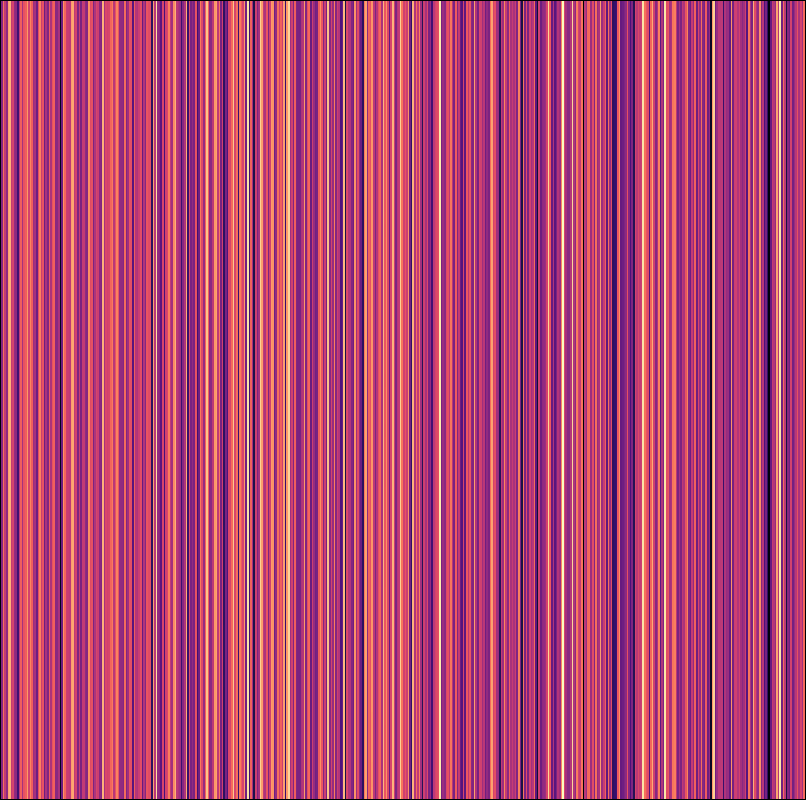
\includegraphics[width=\linewidth]{Attention_Map_RALA_CF.pdf}
        \caption{RALA-CF (RALA).}
        \label{fig:attn_rala}
    \end{subfigure}
    \caption{Token-wise attention maps at the last encoder stage
    ($N{=}512$ tokens on the x-axis, $d{=}64$ channels on the y-axis) for the
    baseline ChangeFormer and the proposed RALA-ChangeFormer.
    Colors represent normalized attention intensity, where darker values
    indicate low attention response and brighter (purple) values indicate higher
    attention. The maps are shown for qualitative comparison only, illustrating
    that RALA preserves non-collapsing spatial attention patterns comparable to
    MHSA \cite{acuna2026efficient}.}
    \label{fig:attn_maps}
\end{figure}

% ── Qualitative Visual Analysis (new in journal version) ─────────────────────
\subsection{\journal{Qualitative Visual Analysis}}
\label{subsec:qualitative}

\journal{%
Figures~\ref{fig:qual_levir_plus}--\ref{fig:qual_s2looking} present qualitative
change detection results on all four extended benchmarks: LEVIR-CD+, SYSU-CD,
WHU-CD, and S2Looking.
Each figure presents a grid of four test samples~(rows) across five columns:
Pre-change image~(A), Post-change image~(B), Ground Truth mask, Model
Prediction, and a four-colour Error Map encoding True Positives~(TP, white),
True Negatives~(TN, black), False Positives~(FP, red), and False
Negatives~(FN, blue).
This layout directly mirrors the output of the \texttt{qualitative\_comparison.py}
pipeline script.%
}

\begin{figure}[t]
    \centering
    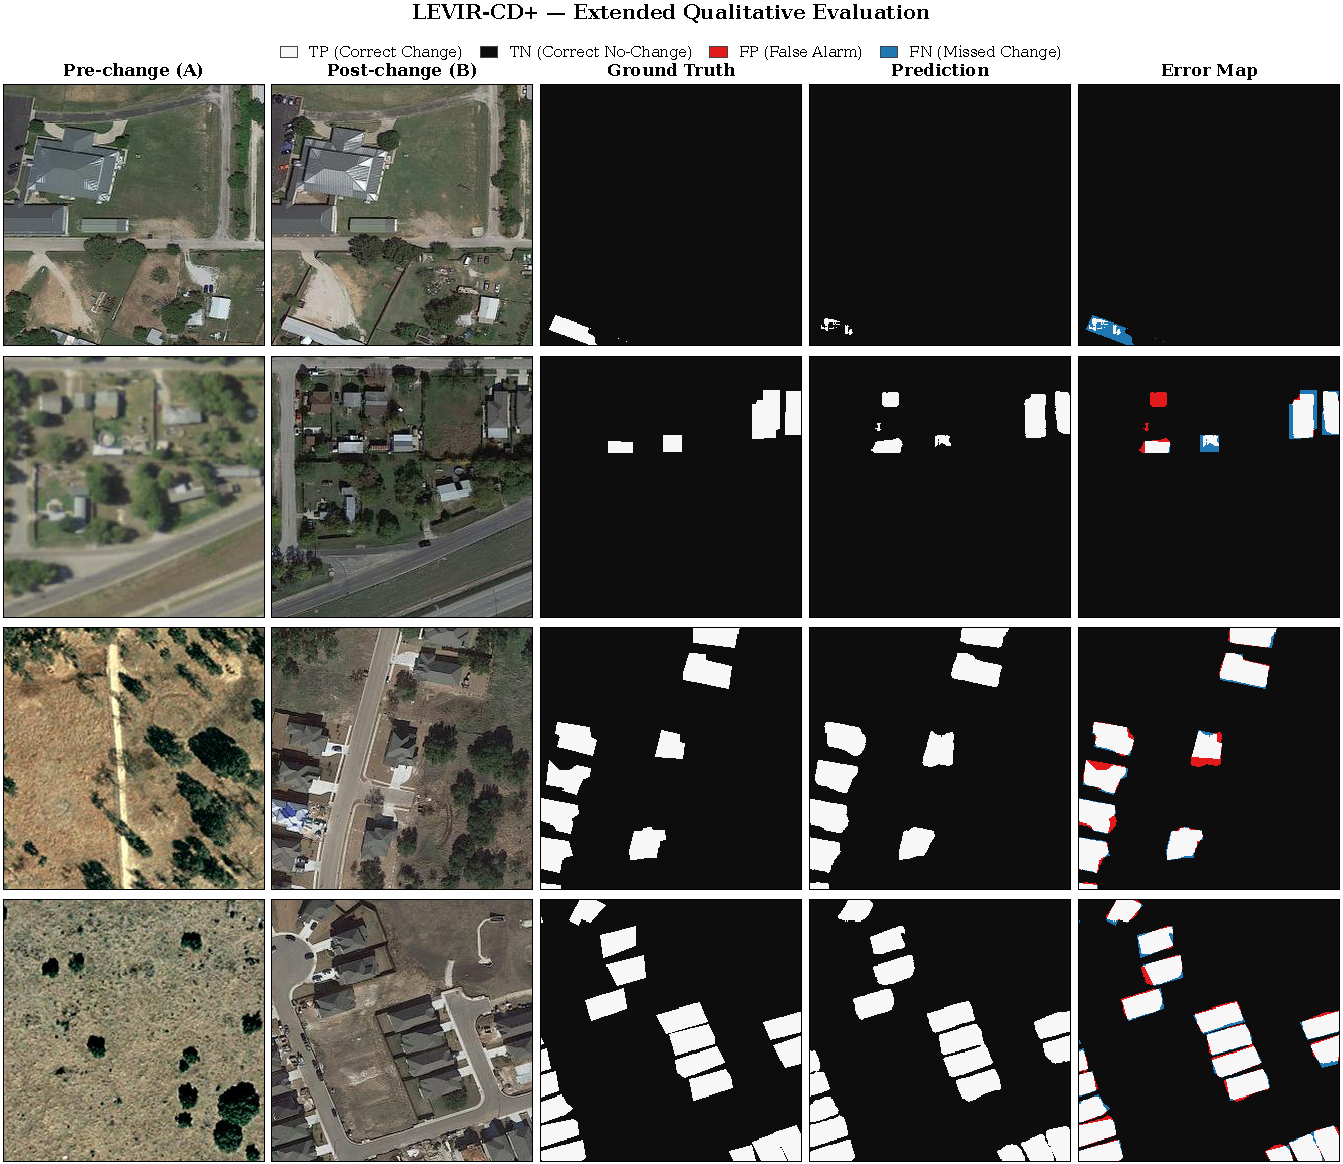
\includegraphics[width=\linewidth]{qualitative_LEVIR_CDPlus.pdf}
    \caption{\journal{Qualitative results on LEVIR-CD+ (four test samples).
    Columns: Pre-change~(A) $|$ Post-change~(B) $|$ Ground Truth $|$
    Prediction $|$ Error Map
    [TP\,=\,white, TN\,=\,black, FP\,=\,red, FN\,=\,blue].
    RALA-ChangeFormer correctly delineates the majority of newly constructed
    building footprints; residual errors concentrate along building boundaries
    and in structurally ambiguous mixed-use zones \cite{acuna2026efficient}.}}
    \label{fig:qual_levir_plus}
\end{figure}

\begin{figure}[t]
    \centering
    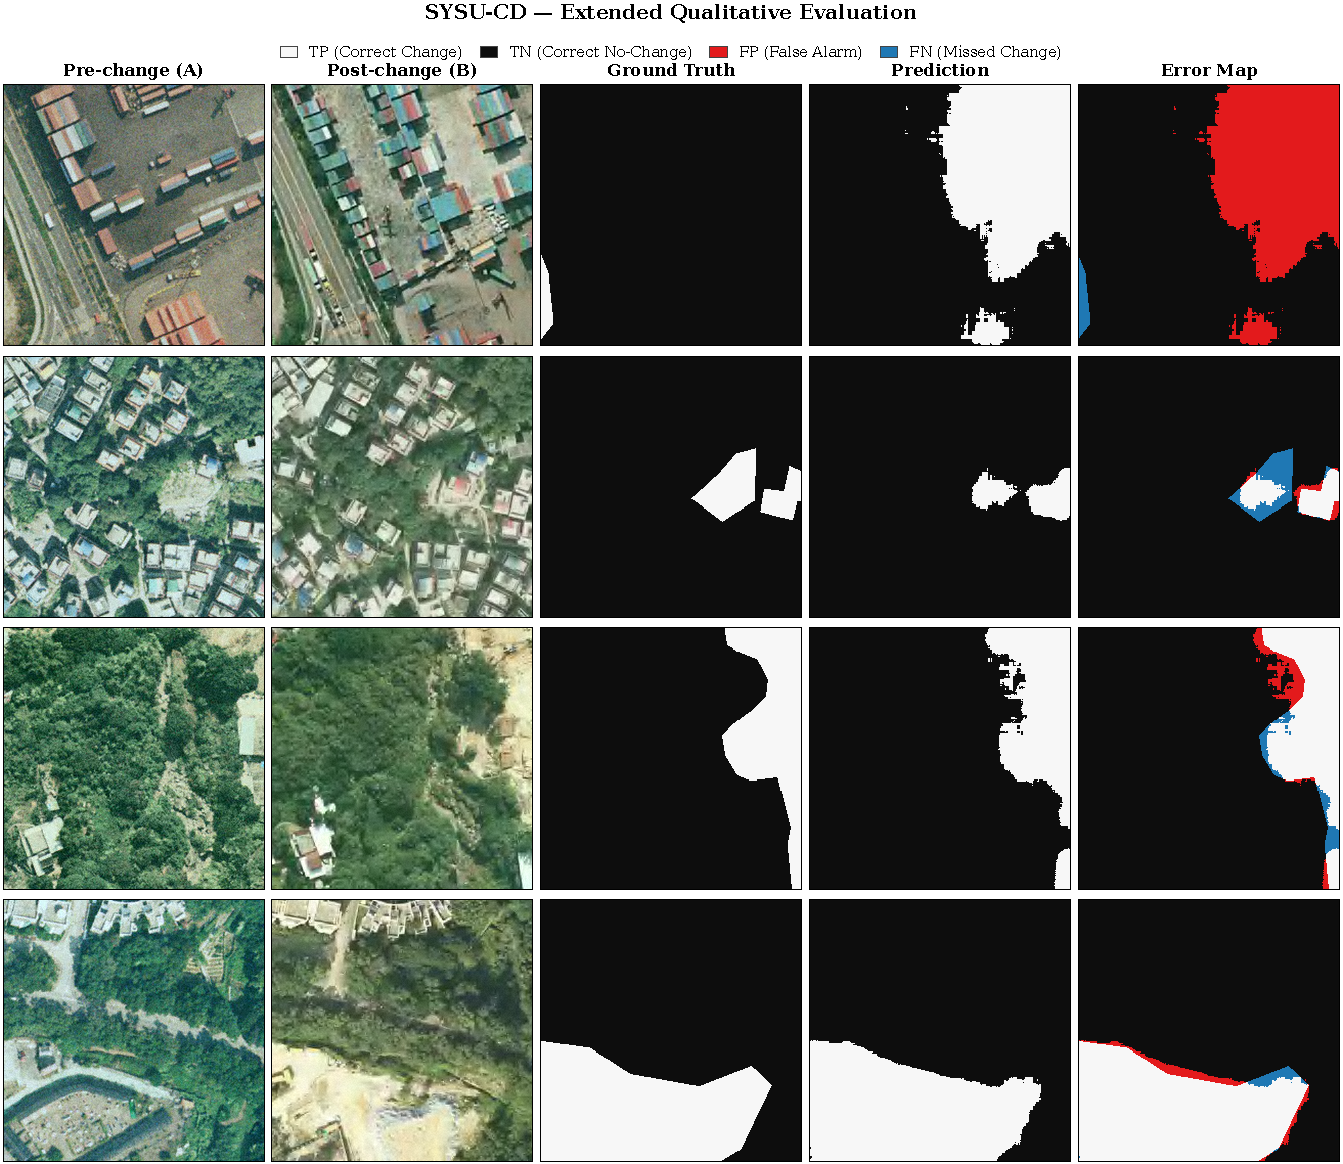
\includegraphics[width=\linewidth]{qualitative_SYSU_CD.pdf}
    \caption{\journal{Qualitative results on SYSU-CD (four test samples).
    Columns: Pre-change~(A) $|$ Post-change~(B) $|$ Ground Truth $|$
    Prediction $|$ Error Map
    [TP\,=\,white, TN\,=\,black, FP\,=\,red, FN\,=\,blue].
    The model detects large-area construction and road changes correctly.
    False alarms~(red) appear predominantly in vegetated buffer zones where
    seasonal spectral variation superficially resembles structural change \cite{acuna2026efficient}.}}
    \label{fig:qual_sysu}
\end{figure}

\begin{figure}[t]
    \centering
    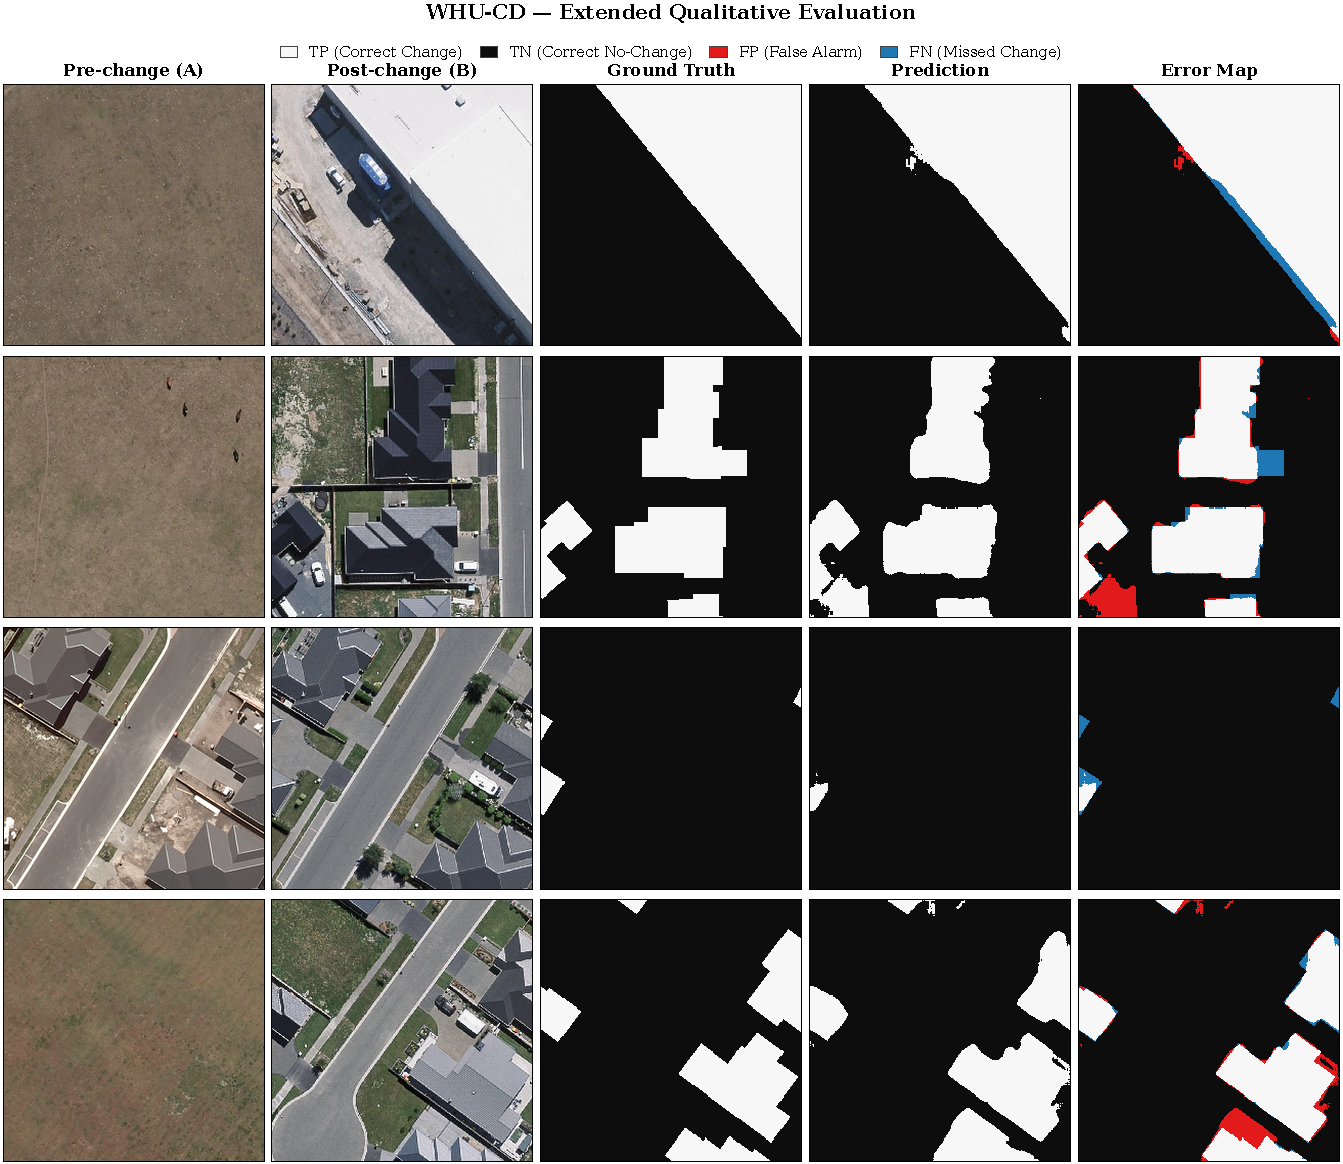
\includegraphics[width=\linewidth]{qualitative_WHU_CD.pdf}
    \caption{\journal{Qualitative results on WHU-CD (four test samples).
    Columns: Pre-change~(A) $|$ Post-change~(B) $|$ Ground Truth $|$
    Prediction $|$ Error Map
    [TP\,=\,white, TN\,=\,black, FP\,=\,red, FN\,=\,blue].
    The centimetre-resolution ($0.3\,\mathrm{m}$) nadir-view imagery enables
    sharp boundary delineation: RALA-ChangeFormer achieves $F_1=87.85\%$ with a
    low false-positive rate. Residual errors concentrate in high-density building
    clusters where adjacent footprints merge under the model's boundary
    discrimination capacity, producing localised false negatives at shared
    building edges \cite{acuna2026efficient}.}}
    \label{fig:qual_whu}
\end{figure}

\begin{figure}[t]
    \centering
    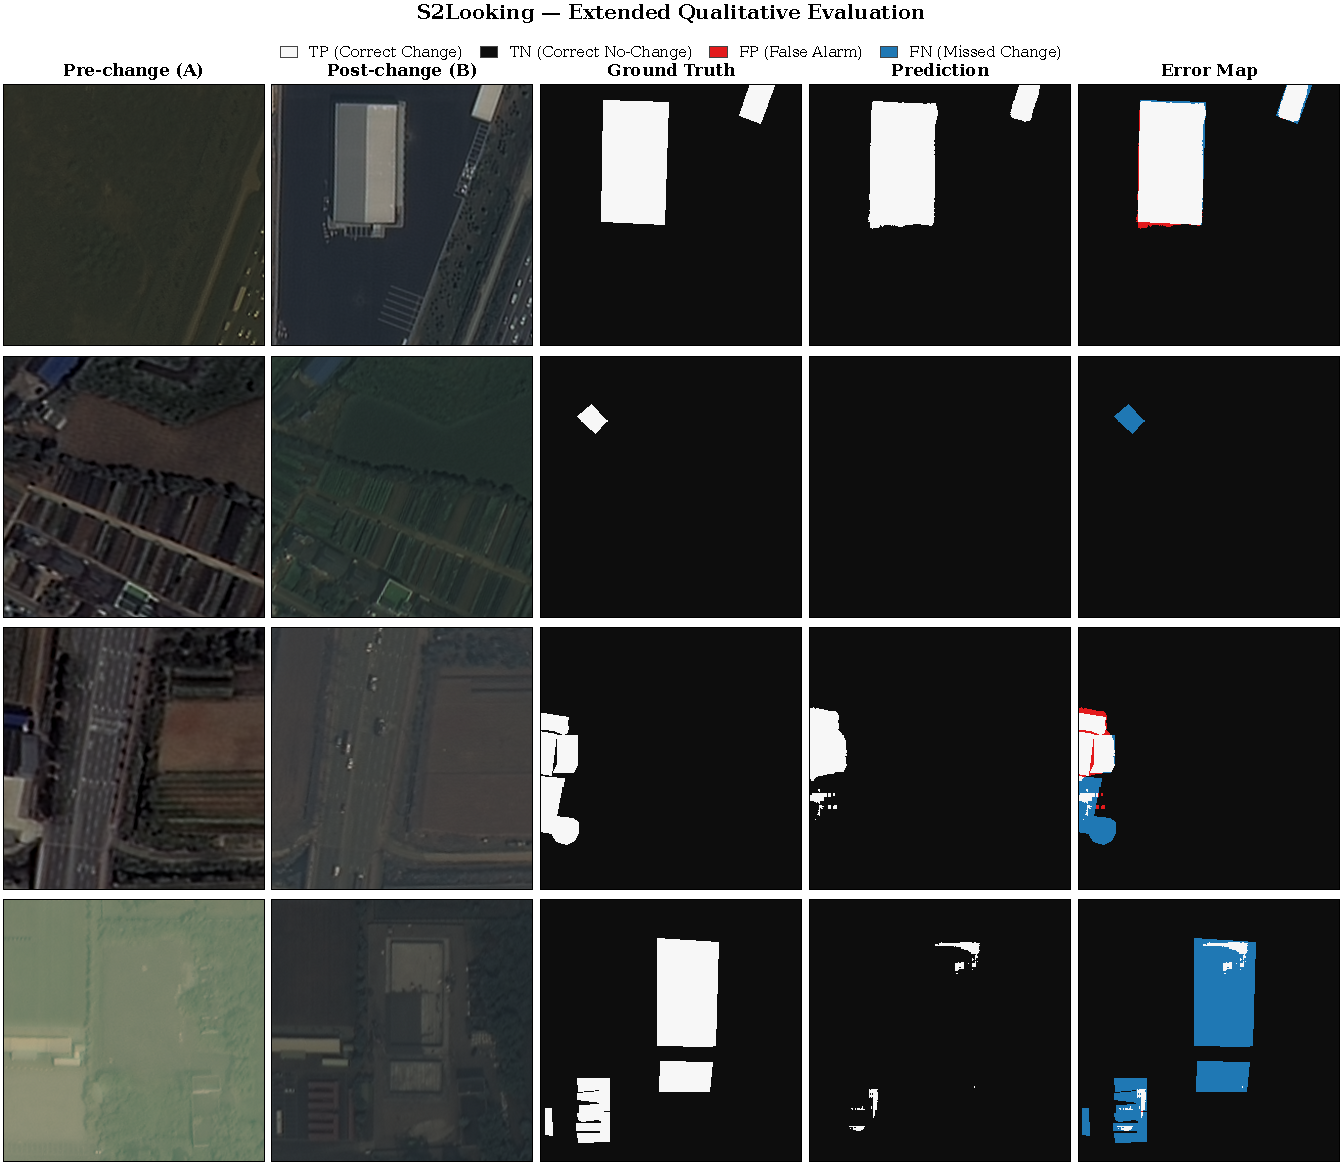
\includegraphics[width=\linewidth]{qualitative_S2Looking.pdf}
    \caption{\journal{Qualitative results on S2Looking (four test samples).
    Columns: Pre-change~(A) $|$ Post-change~(B) $|$ Ground Truth $|$
    Prediction $|$ Error Map
    [TP\,=\,white, TN\,=\,black, FP\,=\,red, FN\,=\,blue].
    The oblique side-looking acquisition geometry introduces apparent positional
    shifts of rooftop boundaries between temporal acquisitions due to parallax,
    producing systematic false negatives~(blue) wherever building edges are
    displaced. Shadow cast by tall structures at non-nadir viewing angles
    generates additional false positives~(red), jointly explaining the low
    recall ($53.09\%$) that characterises this out-of-distribution
    benchmark \cite{acuna2026efficient}.}}
    \label{fig:qual_s2looking}
\end{figure}

\journal{%
On LEVIR-CD+ (Fig.~\ref{fig:qual_levir_plus}), the dominant failure pattern is
boundary under-segmentation: thin false-negative halos appear around correctly
detected building footprints, caused by the global $\alpha$-weighted KV pooling
smoothing the attention response at change/no-change interfaces.
On SYSU-CD (Fig.~\ref{fig:qual_sysu}), systematic false alarms arise in
vegetated and riparian areas, where seasonal greenery fluctuations produce
spectral signatures similar to structural change under binary supervision.
WHU-CD (Fig.~\ref{fig:qual_whu}) exhibits the cleanest error maps across all
four datasets: the nadir-view geometry and high-precision annotations allow the
model to localise building footprints with sharp boundaries; the few remaining
errors concentrate at the edges of densely packed building clusters, where
adjacent footprints merge into ambiguous connected regions.
S2Looking (Fig.~\ref{fig:qual_s2looking}) presents the starkest failure profile:
false negatives dominate the error maps, with blue regions systematically
outlining entire building boundaries; this is a direct consequence of the oblique
acquisition geometry, which displaces rooftop projections relative to the
ground-level annotations and creates spatially inconsistent features that the
LEVIR-CD-pretrained encoder cannot reliably match across time steps.%
}

% ── Statistical Training Dynamics (new in journal version) ───────────────────
\subsection{\journal{Statistical Training Dynamics}}
\label{subsec:dynamics}

\journal{%
Figure~\ref{fig:learning_curves} shows the training and validation mF1 curves
for the four extended benchmarks over the full training duration, as generated
by the \texttt{parse\_results.py} pipeline script.
Each panel marks the best validation epoch~($\star$) and the test F1
(dashed horizontal line).%
}

\begin{figure}[t]
    \centering
    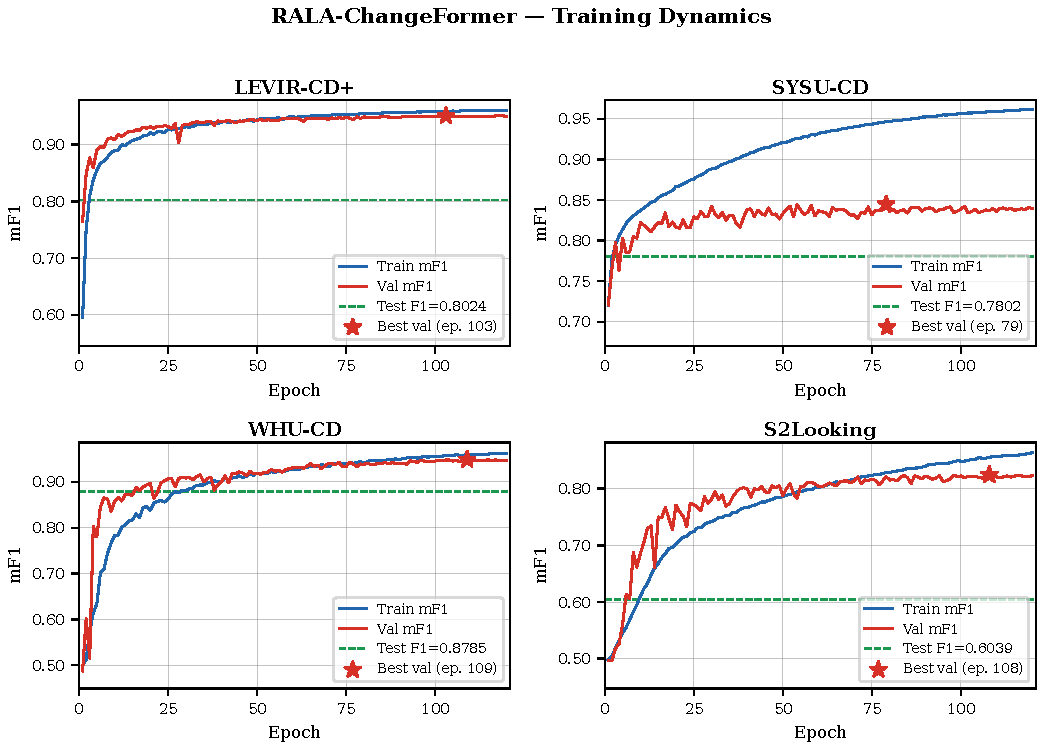
\includegraphics[width=\linewidth]{learning_curves.pdf}
    \caption{\journal{RALA-ChangeFormer training dynamics on the four extended
    benchmarks (LEVIR-CD+, SYSU-CD, WHU-CD, S2Looking).
    Blue: train mF1; red: validation mF1; green dashed: test F1;
    $\star$: best validation checkpoint.
    WHU-CD converges rapidly with minimal train/val divergence.
    S2Looking shows high variance and the largest train-to-test gap,
    reflecting the distributional shift introduced by side-looking geometry \cite{acuna2026efficient}.}}
    \label{fig:learning_curves}
\end{figure}

\journal{%
WHU-CD exhibits the fastest and most stable convergence: validation mF1 rises
steeply within the first 20 epochs, plateaus with minimal overfitting, and the
test F1 closely tracks the validation best—consistent with the dataset's clean
annotations and low class imbalance.
LEVIR-CD+ and SYSU-CD show moderate convergence rates with gradually widening
train/validation gaps beyond epoch~50, partially mitigated by cosine
learning-rate decay.
S2Looking produces the most turbulent dynamics: high epoch-to-epoch variance in
both curves, the widest train-to-test gap, and a best-validation checkpoint
reached late (typically beyond epoch~70), all consistent with the
out-of-distribution challenge of oblique imagery for a nadir-pretrained model.%
}

\subsection{Limitations}
\label{subsec:limitations}

Despite the advantages demonstrated in Sections~\ref{sec:experiments}
and~\ref{sec:discussion}, the proposed integration of rank-augmented linear
attention exhibits several limitations that contextualize its practical impact.

\noindent \textbf{(1) Moderate end-to-end computational gains.} Although rank
augmentation substantially reduces the cost of encoder self-attention, the
overall computational footprint of ChangeFormer is still influenced by
multiscale fusion layers. As shown in Table~\ref{tab:efficiency}, the reduction
in total GFLOPs remains moderate (8--10\%), since attention constitutes only
part of the complete pipeline.


\noindent \textbf{(2) Efficiency improvements grow with token count.} RALA
provides the largest benefits when the number of tokens is high (e.g., 512 or
1024 resolution). At lower input sizes such as $256\times256$, improvements are
measurable but less pronounced, which limits impact for applications operating
strictly at small patch resolutions.

\noindent \textbf{(3) Limited impact on model expressiveness beyond attention.}
While RALA mitigates the low-rank collapse common in linear attention and
preserves segmentation performance, it does not enhance the expressive capacity
of non-attention modules such as convolutional encoders or decoder fusion
layers. As a result, the overall accuracy remains bounded by the
representational capacity of the original ChangeFormer architecture.

\noindent \textbf{(4) Limited evaluation on independent acquisition domains.}
The experimental evaluation follows the standard training and testing protocols
of LEVIR-CD and DSIFN-CD, where splits are spatially disjoint but not fully
independent in terms of acquisition conditions or geographic regions. While this
work focuses on computational scalability and efficiency under commonly adopted
BCD benchmarks, the generalization of RALA-ChangeFormer to unseen acquisition
domains (e.g., cross-region or cross-sensor settings) remains an open question.
Evaluating rank-augmented linear attention under fully independent data
distributions is a promising direction for future work.

\journal{\noindent \textbf{(5) Vulnerability to oblique geometry and
illumination variation.}
Two distinct acquisition-domain failures emerge from the extended evaluation.
First, side-looking perspective distortions (S2Looking, $F_1=60.39\%$,
Rec$=53.09\%$): the parallax displacement of rooftop boundaries between
temporal acquisitions produces large false-negative regions that rank-augmented
attention cannot compensate for through feature reweighting, since the
underlying spatial misalignment is geometric rather than representational.
Second, multi-temporal illumination and seasonal variation (SYSU-CD,
Rec$=74.34\%$): the nine-year acquisition window introduces illumination angle
shifts, seasonal vegetation cycles, and atmospheric differences that cause
phenological spectral changes to be confused with structural changes under
binary supervision. Both failure modes point to the absence of explicit temporal
alignment or domain-normalisation stages in the current architecture.}

\journal{\noindent \textbf{(6) Performance ceiling set by encoder backbone
capacity.}
Across all six datasets, the accuracy of RALA-ChangeFormer closely tracks the
ChangeFormer baseline, confirming that the primary representational bottleneck
lies in the shared SegFormer-B2 encoder rather than in the attention
formulation. The encoder's ADE20K pre-training provides a strong prior for
nadir-view urban structures but a weak one for side-looking or seasonally
variable imagery. Upgrading to SegFormer-B4/B5 or fine-tuning on
domain-specific remote sensing data would likely yield larger accuracy gains
than further refinement of the linear attention mechanism.
Competitive SOTA models such as ChangeMamba~\cite{Chen2024ChangeMamba}
integrate more powerful sequence modelling (selective state spaces) alongside
stronger encoders, confirming that the attention type alone does not determine
the performance ceiling.}

\medskip
\noindent  Overall, although the proposed integration offers practical
advantages in memory efficiency, scalability, and batch-size flexibility, it
does not eliminate the structural constraints inherent to hierarchical
encoder--decoder architectures. These considerations frame the scope of
improvements achieved by substituting MHSA with rank-augmented linear attention.

% =============================================================================
%  6. CONCLUSION  (verbatim from conference + one new paragraph at end)
% =============================================================================
\section{Conclusion}
\label{sec:conclusion}

This work introduced \textbf{RALA-ChangeFormer}, an efficient variant of
ChangeFormer in which the multi-head self-attention modules of the
\textbf{encoder} are replaced with rank-augmented linear attention. All
remaining components of the architecture, including the convolutional backbone,
feed-forward layers, and the lightweight MLP decoder, remain unchanged. The
goal of this modification is to alleviate the quadratic cost of MHSA in
high-token regimes while preserving the representational capacity required for
multi-temporal building change detection.

Experimental evaluations on LEVIR-CD and DSIFN-CD show that RALA-ChangeFormer
maintains segmentation accuracy comparable to the baseline model, confirming
that the rank-augmented KV buffer is sufficiently expressive for bi-temporal
spatial-temporal reasoning. Importantly, unlike previous linear-attention
formulations, RALA avoids the low-rank collapse typically observed in dense
prediction tasks, as further illustrated by the qualitative attention-map
comparisons.

From a computational perspective, the proposed encoder-level integration yields
consistent reductions in attention-related FLOPs and peak GPU memory usage, and
increases feasible batch sizes, particularly at higher resolutions where
attention costs dominate. These improvements enhance practical scalability under
fixed memory budgets, enabling the model to process more patches per iteration
and to support efficient training in high-resolution or large-batch settings
without increasing hardware requirements. Overall, the results demonstrate that
RALA-ChangeFormer provides a favorable accuracy-efficiency trade-off for VHR
change detection, preserving predictive behaviour while reducing resource
demands.

Rather than proposing a novel change detection formulation, this work aims to
empirically assess whether modern linear-attention mechanisms can be integrated
into hierarchical bi-temporal change detection architectures without degrading
performance, and to quantify the resulting efficiency-accuracy trade-offs. In
this context, several promising directions remain for future work. One avenue is
to explore adaptive or data-dependent strategies that refine the rank selection
in RALA, potentially drawing on matrix reconstruction techniques such as SVD to
further enhance representational diversity. Another promising direction is the
integration of RALA into multi-scale or multi-task BCD frameworks, enabling a
more robust evaluation of its generalization capacity across heterogeneous
settings. Finally, with generative approaches—such as diffusion and
flow-matching models—emerging as powerful alternatives for BCD, a key
opportunity lies in developing memory-efficient attention formulations that can
be embedded into these computationally demanding architectures.

\journal{%
The six-dataset cross-domain extension reported in this journal version
(Table~\ref{tab:master}) reinforces the efficiency argument while revealing
concrete accuracy frontiers that future work must address. Four prioritised
directions emerge from this analysis.

\noindent\textbf{(a) Dynamic rank adaptation.}
Building on the SVD-based direction outlined above, introducing a
data-dependent rank selection strategy—estimating the intrinsic dimensionality
of the KV buffer via an online lightweight step—could allocate higher rank
capacity to geometrically complex or temporally inconsistent patches while
compressing representation for homogeneous no-change regions, targeting the
S2Looking gap directly.

\noindent\textbf{(b) Geometric perspective alignment for oblique imagery.}
The S2Looking results ($F_1=60.39\%$) identify viewpoint-induced parallax as
the dominant open failure mode. Incorporating a deformable or
perspective-aware attention module upstream of the RALA encoder, or a
homography-based pre-alignment stage, would provide the geometric invariance
that rank augmentation cannot deliver alone.

\noindent\textbf{(c) Integration into and competition with current SOTA.}
State-of-the-art models such as ChangeMamba~\cite{Chen2024ChangeMamba} achieve
superior accuracy by combining stronger backbones with selective state-space
sequence modelling. Integrating the RALA mechanism within such architectures
would allow the same efficiency gains while benefiting from their stronger
representational priors, positioning rank-augmented linear attention as a
complementary component rather than a standalone solution.

\noindent\textbf{(d) Heterogeneous and Latin American datasets.}
The six benchmarks evaluated here—despite their diversity—share a geographic
and morphological bias toward East Asian and Australasian urban environments
with relatively regular planning patterns and building footprint geometries.
A critical open challenge is adapting BCD models to the informal urban growth,
mixed-use land parcels, and heterogeneous building materials of Latin American
cities such as Lima, Bogotá, and São Paulo, where informal settlements can
expand rapidly with irregular geometries that diverge substantially from the
structured footprints in LEVIR-CD or WHU-CD. Constructing benchmark datasets
targeting these environments—using open imagery from platforms such as INPE
or Copernicus EMS—would provide a more demanding and globally representative
evaluation for efficient BCD models and more directly address the sustainability
challenges of urban monitoring in the Global South.%
}

% =============================================================================
%  ACKNOWLEDGEMENTS
% =============================================================================
\section*{Acknowledgements}

We gratefully acknowledge the support of the GINIA research group, where this
work was initiated. GINIA provided an academic research environment that
supported the early stages of this work in urban data analysis and covered the
conference registration fee.
\journal{D.\,Quispe Apaza designed and executed the four extended benchmark
experiments (LEVIR-CD+, SYSU-CD, WHU-CD, S2Looking) reported in this journal
version.}

% =============================================================================
%  REFERENCES
% =============================================================================
\bibliographystyle{splncs04}
\bibliography{example}

\end{document}
% ============================================================  END OF FILE
